\begin{figure}[tb]
\begin{center}
%\fbox{\rule{0pt}{2in} \rule{0.9\linewidth}{0pt}}
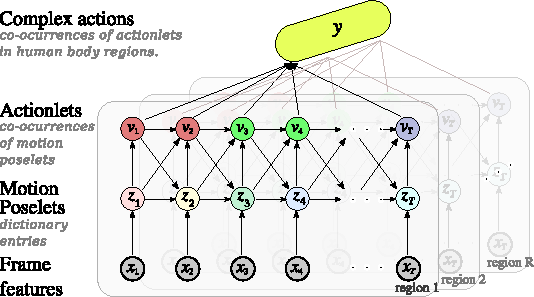
\includegraphics[width=0.99\linewidth]{./Fig/modelo.pdf}
\vspace{-2mm}
\end{center}
\caption{\footnotesize
Graphical representation of our discriminative hierarchical model for 
recognition of composable human activities.
At the top level, activities are represented as compositions of atomic actions that are inferred at
the intermediate level. These actions are in turn compositions of poses at the
lower level, where pose dictionaries are learned from data. Our model also learn
temporal transitions between consecutive poses and actions. Best viewed in
color.}
\label{fig:overview}
\vspace{-4mm}
\end{figure}


In this section, we introduce our model for pose-based recognition of complex 
human actions. Our goal is to provide the model with the capability of 
annotating input videos according to the actions being performed. In 
particular, we are interested in automatically identifying the parts of the body 
that are involved in each action (spatial localization), as well as the temporal 
span of each action (temporal localization). Since we are interested in 
concurrent and composable activities, we would also like to encode multiple 
levels of abstraction, so that we can encode poses, actions, and their 
compositions. Therefore, we develop a hierarchical compositional framework for 
modeling and recognizing complex human actions.

One of the key contributions of our model is its capability of spatially 
localizing the body regions that are involved in the execution of each action, 
\emph{both at training and testing time}. This is, our training process does not 
require careful spatial annotation and localization of actions in the training 
set. Instead, it uses temporal annotations of actions so 
that, at test time, it can discover the spatial and temporal span, as well as, 
the specific configuration of the main body regions executing each action. In 
the following, we introduce the components of our model and the training 
process that achieves this goal.

\begin{figure}[tb]
\begin{center}
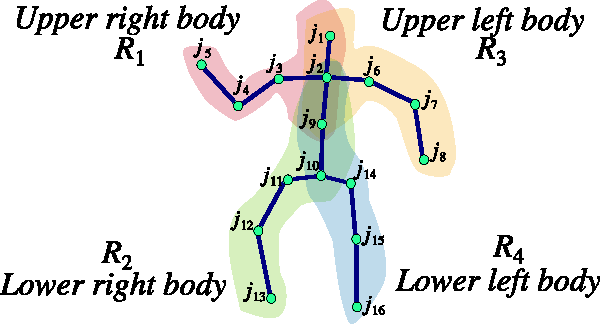
\includegraphics[width=0.8\linewidth]{./Fig/fig_joints_limbs_region.pdf}
\vspace{-2mm}
\end{center}
\caption{
\footnotesize
Skeleton representation used for splitting the human body into a set of 
spatial regions.}
\label{fig:skeleton_limbs_regions}
\vspace{-4mm}
\end{figure}

\subsection{Body regions}
We divide the body pose into $R$ fixed spatial regions and independently compute 
a pose feature vector for each region. Fig. \ref{fig:skeleton_limbs_regions} 
illustrates the case when $R = 4$ that we use in all our experiments. Our body 
pose feature vector consists of the concatenation of two descriptors. At frame 
$t$ and region $r$, a descriptor $x^{g}_{t,r}$ encodes geometric information 
about the spatial configuration of body joints, and a descriptor $x^{m}_{t,r}$ 
encodes local motion information around each body joint position. Following 
\cite{Lillo2014}, our geometric descriptor is based on angles between segments 
connecting two joints, and angles between these segments and a plane formed by 
three joints (see \cite{Lillo2014} for details). Following \cite{WangCVPR2011}, 
our motion descriptor is based on tracking motion trajectories of key points, in 
our case, joint positions. Specifically, we compute at each joint location a HOF 
using RGB patches centered at the joint location for a temporal window of 15 
frames. At each joint location, this produces a 108-dimensional descriptor,  
that we concatenate across all joints inside a region to obtain our motion descriptor. Finally, 
to reduce dimensionality, we apply PCA to transform the concatenated descriptor 
into a 20-dimensional vector, keeping the dimensionality of our final descriptor 
relatively low.


\subsection{Hierarchical compositional model}

We propose a compositional hierarchical model that spans three semantic levels. 
At the top level, our model assumes that each complex action is composed of a 
temporal and spatial arrangement of a known set of $A$ atomic actions, where 
each input video has a single complex action label. Similarly, at the 
intermediate level, our model assumes that each atomic action is composed of a 
temporal arrangement of $K$ body poses, where $K$ is a parameter of 
our model. Finally, at the bottom level, our model identifies local body poses 
using a bank of linear classifiers that are applied to the incoming frame 
descriptors. 

Similarly to previous works \cite{Lillo2014, Taralova:EtAl:2014}, we build 
each layer of our hierarchical model on top of BoW 
representations. To this end, at the bottom level of our hierarchy, and for 
each body region, we learn a dictionary of body part configurations that we 
refer to as motion poselets. Similarly, at the mid-level of our hierarchy, and 
for each atomic action, we learn a dictionary of representative action 
configurations that we refer to as actionlets. At each of these levels, 
spatio-temporal activations of the respective dictionary words are used 
to obtain the corresponding histogram encoding the BoW representation. 
Next two sections provide 
details behind the process to represent and learn the dictionaries of motion 
poselets and actionlets. Here we provide further details of the 
integrated hiearchical model.

We expresses our hierarchical model using an energy formulation. 
Specifically, given a video $D$ with $T$ frames, we
define an energy function for $D$ as:
{\small
\begin{align}\label{Eq_energy}
%\begin{split}
E(D) = & E_{\text{motion poselets}} + E_{\text{motion poselets BoW}} + 
E_{\text{actionlets BoW}} \nonumber \\ 
& + E_{\text{motion poselets transition}} + E_{\text{actionlets 
transition}}.
%\end{split}
\end{align}}
With respect to the BoW representations and motion poselet classifiers 
described above, Equation (\ref{Eq_energy}) also 
consider two additional energy potentials that encode information related to 
temporal 
transitions between pairs of motion poselets ($E_{\text{motion poselets 
transition}}$) and 
actionlets ($E_{\text{actionlets transition}}$), respectively. Our goal is to 
maximize $E(D)$, such that, we obtain the 
spatial and temporal arrangement 
of motion poselets and actionlets, as well as, the underlying 
complex action. 

Considering the BoW representations and linear classifiers to identify motion 
poselets, 
the previous energy potentials are given by:
{\small
\begin{align}
\label{eq:motionposelets}E_{\text{motion poselets}}  =  &\sum_{r=1}^R\sum_{t=1}^T  \left[ \sum_{k=1}^K {w^r_k}^\top 
x_{t,r}\delta_{z_{(t,r)},k} + \theta^r \delta_{z_{(t,r)},K+1}\right] \\
E_{\text{motion poselets BoW}} & = \sum_{r=1}^R \sum_{a=1}^A {\beta^r_{a}}^\top 
h^{a}(Z_r,V_r)\\
\label{eq:actionlets_BoW} E_{\text{actionlets BoW}} &=\sum_{r=1}^R {\alpha^r_{y}}^\top h(V_r)  \\
E_{\text{mot. pos. transition}} & = 
\sum_{r=1}^R\sum_{k=1}^{K+1}\sum_{k'=1}^{K+1} \eta^r_{k,k'} 
\sum_{t=1}^{T-1} \delta_{z_{(t-1,r)},k}\delta_{z_{(t,r)},k'}\\ 
\label{eq:actionletstransition}
E_{\text{actionlets transition}} & =\sum_{r=1}^R\sum_{a=1}^A\sum_{a'=1}^A \gamma^r_{a,a'} 
\sum_{t=1}^{T-1} 
\delta_{v_{(t,r)},a}\delta_{v_{(t+1,r)},a'} 
\end{align}
}
In the previous equations, the energy term associated with motion poselets 
$w^r_k$ refers to a set of $K$ linear pose classifiers, applied to frame 
descriptors $x_t^r$, according to the label of the latent variable $z_t^r$. 
Note that there is a special label $K+1$; the role of this label will be 
explained in Section \ref{subsec:garbage_collector}. $\delta_{i,j}$ represents 
the Kronecker delta function. In terms of the energy potential associated to 
the BoW representation for motion poselets, $\beta_a^r$ denotes a set of $A$ 
mid-level classifiers, whose inputs are histograms $h^a(Z_r,V_r)$ of motion 
poselet labels at those frame annotated as actionlet $a$. At the highest level, 
$\alpha^r_{y}$ is a linear classifier  associated to complex action $y$, whose 
input is the histogram of actionlet labels $h(V_r)$. Note that all classifiers 
and labels are referred to a single region $r$; we add the contributions of all 
regions to compute the global energy of the video. The transition terms acts as 
linear classifiers over histograms of temporal transitions of motion poselet 
and temporal transitions of actionlet, respectively.

\subsection{Learning motion poselets}
In our model, motion poselets are learned treating them as latent variables  
during training. Before training, we fix the number of motion poselets 
according to parameter $K$. In every region $r$ we learn an independent 
set of pose classifiers $\{w^r_k\}_{k=1}^K$, initializing the motion poselet 
labels using $k$-means algorithm. Then, we learn pose classifiers jointly with 
actionlets and complex actions classifiers, allowing the model to discover 
discriminative motion poselets useful to detect and recognize complex actions. 
As shown in \cite{Lillo2014} and \cite{Tao2015}, jointly learning linear 
classifiers to identify body parts and atomic actions improves recognition 
rates, so here we follow a similar hierarchical approach, an integrate learning 
of motion poselets with learning of actionlets.     

\subsection{Learning actionlets}
A single linear classifier does not offer enough flexibility to identify actions 
that feature high variability. Consequently, we augment the previous 
hierarchical model to include multiple linear classifiers per action. We create 
two new concepts: \textbf{semantic actions}, that refer to actions \emph{names} 
that compose an activity; and \textbf{actionlets}, that refers to the sequence 
of motion poselets that build an action. The main idea is that action 
annotations in the dataset are associated to semantic actions, whereas for each 
semantic action we learn several actionlet classifiers. This formulation allows 
us to handle the multimodal nature of semantic actions, covering changes in 
motion, pose, or even changes in meaning of the action according to context 
(e.g. the semantic action ``open'' can be associated to opening a can, opening a 
door, etc.). 

Inspired by \cite{Raptis2012}, we first use the \emph{Cattell's Scree test} for 
finding a suitable number of actionlets for every semantic action in an unsupervised fashion. Using 
the semantic action labels, we compute a descriptor for every interval using 
normalized histograms of pose labels. Then, for a particular semantic action 
$u$, we compute the eigenvalues $\lambda_u$ of the affinity matrix of the 
semantic action descriptors, using $\chi^2$ distance. For each semantic action 
$u \in \{1,\dots,U\}$, we find the number of actionlets $G_u$ as $G_u = 
\argmin_i \lambda_{i+1}^2 / (\sum_{j=1}^i \lambda_j) + c\cdot i$, with $c=2\cdot 
10^{-3}$. Finally, we cluster the descriptors corresponding to each semantic 
action using k-means, using a different number of clusters for each semantic 
action $u$ according to $G_u$. This approach generates non-overlapping actionlets, each associated to a single semantic action.

To transfer the new labels to the model, we define $u(v)$ as the function that, 
given the actionlet label $v$, returns the corresponding semantic action 
label $u$. With respect to Equation (\ref{eq:actionlets_BoW}), the energy for 
the actionlet BoW is replaced by
{\small
\begin{equation}
E_{\text{actionlets BoW}} =  \sum_{r=1}^R\sum_{t=1}^T\sum_{u=1}^U \alpha_{y,u}\delta(u(v_t)=u)
\end{equation}}
where we expand histogram $h(V_r)$ to 
make explicit its dependence to the mapping function $u(v)$. A 
dictionary of actionlets provide a richer representation for actions, 
where several actionlets will map to a single semantic action. This 
behavior resembles a max-pooling operation, where at inference time we will 
choose the set of actionlets that best describe the performed actions in the 
video, keeping the semantics of the original labels. 

\subsection{Motion poselets garbage collector}
\label{subsec:garbage_collector}
The model in \cite{Lillo2014} uses all poses to feed action classifiers. Our 
intuition is that only a subset of poses in each video are really discriminative 
or informative for the actions being performed. Low-scored motion poselets 
could  degrade the pose classifiers during training, decreasing their 
performance. 
We include a mechanism to handle those low-scored 
frames leading to more discriminative motion poselet classifiers. 
We call this contribution as \emph{motion poselets garbage collector}, since it 
handles all low-scores motion poselets and group them. We use a special pose 
entry $K+1$ to identify the non-informative poses, which in practice are 
associated to a score lower than $\theta_r$, as shown in Equation 
(\ref{eq:motionposelets}).



\subsection{Learning} \label{subsec:learning}

[IL: These are notes, don't evaluate it yet]

The loss function $\Delta((y_i,V_i),(y,V))$ can no longer depend in the value of $V_i$, since it is now a latent variable. But, as we do know the time span of the actions in all videos, we can compute a list $A_t$ of possible actions for frame $t$, and transform the original loss function into
\begin{equation}
\Delta(y_i,(y,V)) = \lambda_y(y_i \ne y) + \lambda_v\frac{1}{T}\sum_{t=1}^T \delta(v_t \notin A_t)
\end{equation}
and use the same group of actions for each frame to impute the labels of actions and poses for each frame during the inference of latent variables

The model parameters are learned with a Latent Structural SVM formulation, iterating between searching the best assignments of poses $Z$ given the model parameters, and finding the best classifiers given the poses $Z$:
\begin{equation}
 Z_i^* = \max_{Z_i} E(X_i, Z_i, V_i, y_i)
\end{equation} 

\subsection{Inference}
The input to the inference algorithm is a new video sequence with features
$X$. The task is to infer the best activity label $\hat y$ and the best
atomic action labels $\hat V$. Additionally, we also need to estimate latent variables $Z$.
%{\small
\begin{equation}
  \hat y, \hat V, \hat Z = \argmax_{y, V, Z} E(X, Z, V, y)
\end{equation}
%}
We can solve this by the same equations for solving the most violated constraint during learning, setting %as in Equation (\ref{dp_recursion}), using 
$\lambda_i =0$, $i = \{1,2\}$, by exhaustively enumerating all values of activities $y$, and solving for atomic actions assignments $\hat{V}$ and pose assignments $\hat{Z}$ using:
%the following at each step:
%%{\small
%\begin{equation}
% \hat V, \hat Z | y= \argmax_{V,Z} E(X, Z, V, y)
%\end{equation}
%%}
%Therefore, for each possible activity class $y$, we must find $\hat V$ and
%$\hat Z$ using:
%{\small
\begin{equation}
\begin{split}
 \hat{V}, \hat{Z} | y ~ =~ &   \argmax_{V,Z} ~   \sum_{t=1}^T \left( \alpha_{y,v_{t}} 
                  + \beta_{v_{t},z_{t}} + {w_{z_{t}}}^\top x_{t} \delta(z_t \le K)  \right. \\ 
				& \quad\quad \left. \vphantom{{w_{z_{t}}}^\top x_{t}} + \theta \delta(z_t = K+1) + \gamma_{v_{{t-1}},v_t} + \eta_{z_{{t-1}},z_t}  \right). \\
\end{split}
\label{eq:classify_inference}
\end{equation}
%} 






